\documentclass[11pt,a4paper]{article}

\usepackage[a4paper,margin=1in]{geometry}
\usepackage{multicol}
\usepackage{enumitem}
\usepackage{fancyhdr}
\usepackage{setspace}
\usepackage{amsmath}
\usepackage{float}
\usepackage{graphicx}
\usepackage{gvv}
\usepackage{gvv-book}
\usepackage{listings}
\lstset{frame=single, breaklines=true, columns=fullflexible}
\usepackage{caption}
\usepackage[normalem]{ulem}

\pagestyle{fancy}
\fancyhf{}
\fancyhead[L]{GATE 2024}
\fancyhead[C]{\textbf{General Aptitude}}
\fancyfoot[C]{\thepage}

\setlength{\parindent}{0pt}
\setlength{\parskip}{2pt}

\begin{document}

\rule{\columnwidth}{0.3pt}

\textbf{Q. 1 -- Q. 5 carry one mark each.}

\begin{enumerate}
\item If I were you, I \underline{\hspace{2.5cm}} that laptop. It’s much too expensive.\hfill {(GATE EE 2025)}

\begin{multicols}{2}
\begin{enumerate}
\item won’t buy
\item shan’t buy
\item wouldn’t buy
\item would buy
\end{enumerate}
\end{multicols}



\item He \underline{turned a deaf ear} to my request. 

What does the underlined phrasal verb mean?\hfill {(GATE EE 2025)}

\begin{multicols}{2}
\begin{enumerate}
\item ignored
\item appreciated
\item twisted
\item returned
\end{enumerate}
\end{multicols}


\item Choose the most appropriate set of words from the options given below to complete the following sentence:

\begin{quote}
\underline{\hspace{3cm}} \quad \underline{\hspace{3cm}} \quad is a will, \quad \underline{\hspace{3cm}} \quad is a way.
\end{quote}
\hfill {(GATE EE 2025)}
\begin{multicols}{2}
\begin{enumerate}
\item Wear, there, their
\item Were, their, there
\item Where, there, there
\item Where, their, their
\end{enumerate}
\end{multicols}



\item $(x \% \text{ of } y) + (y \% \text{ of } x)$ is equivalent to:\hfill {(GATE EE 2025)}

\begin{multicols}{2}
\begin{enumerate}
\item $2 \%$ of $xy$
\item $2 \%$ of $\frac{xy}{100}$
\item $xy \%$ of 100
\item $100 \%$ of $xy$
\end{enumerate}
\end{multicols}



\item The sum of the digits of a two digit number is 12. If the new number formed by reversing the digits is greater than the original number by 54, find the original number.\hfill {(GATE EE 2025)}

\begin{multicols}{2}
\begin{enumerate}
\item 39
\item 57
\item 66
\item 93
\end{enumerate}

\end{multicols}

\end{enumerate}


\noindent \textbf{Q.6 -- Q.10 carry two marks each.}

\begin{enumerate}[leftmargin=0pt,label=\textbf{Q.\arabic*}, resume]

\item Two finance companies, P and Q, declared fixed annual rates of interest on the amounts invested with them. The rates of interest offered by these companies may differ from year to year. Year-wise annual rates of interest offered by these companies are shown by the line graph provided below.


\begin{figure}
    \centering
    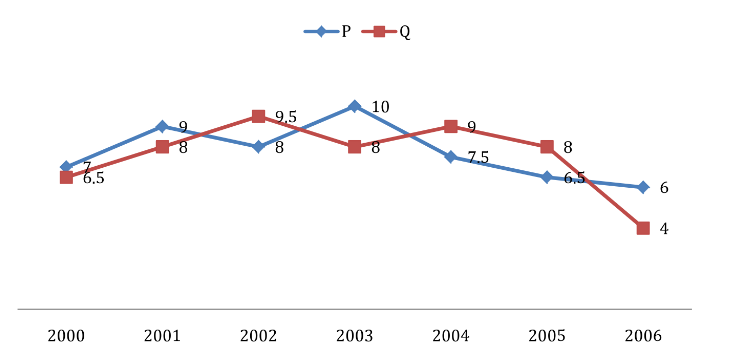
\includegraphics[width=0.9\columnwidth]{figs/imageQ6.png}
    \caption{Year-wise annual rates of interest offered by companies P and Q.}
    \label{fig:q6-rates}
\end{figure}

\newpage
If the amounts invested in the companies, P and Q, in 2006 are in the ratio 8:9, then the amounts received after one year as interests from companies P and Q would be in the ratio:\hfill {(GATE EE 2025)}

\begin{multicols}{2}
\begin{enumerate}
\item 2 : 3
\item 3 : 4
\item 6 : 7
\item 4 : 3
\end{enumerate}
\end{multicols}


\end{enumerate}
\fancyhead[C]{Ecology -- EY}

\begin{enumerate}[leftmargin=*,label=\textbf{Q.\arabic*},resume]
\item Today, we consider Ashoka as a great ruler because of the copious evidence he left behind in the form of stone carved edicts. Historians tend to correlate greatness of a king at his time with the availability of evidence today.

Which of the following can be logically inferred from the above sentences?\hfill {(GATE EE 2025)}
\begin{enumerate}
\item Emperors who do not leave significant sculpted evidence are completely forgotten.
\item Ashoka produced stone carved edicts to ensure that later historians will respect him.
\item Statues of kings are a reminder of their greatness.
\item A king’s greatness, as we know him today, is interpreted by historians.
\end{enumerate}

\item Fact 1: Humans are mammals.\\ 
Fact 2: Some humans are engineers.\\ 
Fact 3: Engineers build houses.

If the above statements are facts, which of the following can be logically inferred?\hfill {(GATE EE 2025)}

\begin{enumerate}[label=\roman*.]
\item All mammals build houses.
\item Engineers are mammals.
\item Some humans are not engineers.
\end{enumerate}

\begin{multicols}{2}
\begin{enumerate}
\item II only
\item III only
\item I, II and III
\item I only
\end{enumerate}
\end{multicols}

\item A square pyramid has a base perimeter $x$, and the slant height is half of the perimeter. What is the lateral surface area of the pyramid?\hfill {(GATE EE 2025)}

\begin{multicols}{2}
\begin{enumerate}
\item $x^2$
\item $0.75 x^2$
\item $0.50 x^2$
\item $0.25 x^2$
\end{enumerate}
\end{multicols}

\item Ananth takes 6 hours and Bharath takes 4 hours to read a book. Both started reading copies of the book at the same time. After how many hours is the number of pages \textbf{to be} read by Ananth, twice that \textbf{to be} read by Bharath? Assume Ananth and Bharath read all the pages with constant pace.\hfill {(GATE EE 2025)}

\begin{multicols}{2}
\begin{enumerate}
\item 1
\item 2
\item 3
\item 4
\end{enumerate}
\end{multicols}
\begin{center}
  \textbf{END OF QUESTION PAPER}  
\end{center}

\end{enumerate}
% --- Page 1/11, Ecology section start ---
\newpage
\fancyhead[C]{Ecology -- EY}

\begin{center}
    {\Large \textbf{Ecology -- EY}}
\end{center}
\rule{\columnwidth}{0.4pt}


\noindent \textbf{Q. 1 -- Q. 25 carry one mark each.}

\begin{enumerate}[leftmargin=*,label=\textbf{Q.\arabic*}]

\item Different kinds of limbs, such as the wings of birds and bats, and the flippers of turtles, whales and dolphins, have the same underlying skeletal structure. This is an example of:\hfill {(GATE EE 2025)}
\begin{multicols}{2}
\begin{enumerate}
\item Analogy
\item Convergence
\item Homology
\item Genetic drift
\end{enumerate}
\end{multicols}

\item Forests with a high density of native conifer trees are found in:\hfill {(GATE EE 2025)}
\begin{multicols}{2}
\begin{enumerate}
\item Gujarat
\item Haryana
\item Himachal Pradesh
\item Odisha
\end{enumerate}
\end{multicols}

\item Ozone layer depletion, since the 1970s, is primarily attributed to:\hfill {(GATE EE 2025)}
\begin{multicols}{2}
\begin{enumerate}
\item carbon dioxide
\item chlorofluorocarbons
\item global warming
\item UV radiation
\end{enumerate}
\end{multicols}

\item The evolution of the amniotic egg in reptiles allowed them to:\hfill {(GATE EE 2025)}
\begin{multicols}{2}
\begin{enumerate}
\item colonize dry terrestrial environments
\item give birth to live young
\item lay eggs in water and on land
\item live in aquatic environments
\end{enumerate}
\end{multicols}

\item Which of the following phyla are most closely related to chordates?\hfill {(GATE EE 2025)}
\begin{multicols}{2}
\begin{enumerate}
\item Annelida
\item Arthropoda
\item Echinodermata
\item Mollusca
\end{enumerate}
\end{multicols}

\item Limb lengths were measured for 50 individuals from a population of lizards and the sample variance was calculated to be 64 cm$^2$. The standard deviation for this sample is \underline{\hspace{2cm}} cm.\hfill {(GATE EE 2025)}
\item Most terrestrial ecosystems have a pyramidal structure of standing biomass across trophic levels where biomass of producers $>$ primary consumers $>$ secondary consumers $>$ tertiary consumers. However, some aquatic ecosystems have an inverted pyramidal structure where the standing biomass of producers $<$ primary consumers. An explanation for this is:\hfill {(GATE EE 2025)}
\begin{multicols}{2}
\begin{enumerate}
\item greater efficiency of primary consumers in aquatic ecosystems
\item high turnover rates of aquatic producers relative to consumers
\item low nutrient concentrations in aquatic ecosystems
\item very high light limitation in aquatic ecosystems
\end{enumerate}
\end{multicols}

\item In an experiment, a PhD student found that the traits, flower colour and seed size, did not follow Mendel’s Law of Independent Assortment. A possible explanation for this observation is:\hfill {(GATE EE 2025)}
\begin{multicols}{2}
\begin{enumerate}
\item co-dominance between alleles
\item incomplete dominance
\item linkage between the traits
\item loci on different chromosomes
\end{enumerate}
\end{multicols}

\item Which of the following invertebrates has the lowest gut length:body length ratio?\hfill {(GATE EE 2025)}
\begin{multicols}{2}
\begin{enumerate}
\item dragonflies
\item grasshoppers
\item leaf hoppers
\item termites
\end{enumerate}
\end{multicols}

\item Allopatric speciation occurs when two populations diverge because of geographical separation. Rates of allopatric speciation are likely to be higher in:\hfill {(GATE EE 2025)}

\begin{enumerate}
\item marine organisms with active dispersal
\item marine organisms with passive dispersal
\item terrestrial organisms with high dispersal ability
\item terrestrial organisms with low dispersal ability
\end{enumerate}

\end{enumerate}
\begin{enumerate}[leftmargin=*,label=\textbf{Q.\arabic*},resume]

\item For nearly 200 years, biogeographers have noted that the tropics have more terrestrial species than temperate regions. Which of the following is \textbf{NOT} a plausible explanation for this pattern?\hfill {(GATE EE 2025)}
\begin{enumerate}
\item Diversification rates are higher in the tropics
\item Energy inputs are higher in the tropics
\item There is greater land area in the tropics
\item Tropical species have greater climatic tolerance
\end{enumerate}

\item If the rate of non-synonymous substitution at a locus exceeds that of synonymous substitution, then:\hfill {(GATE EE 2025)}
\begin{enumerate}
\item deleterious mutations are accumulating
\item evolution is not occurring
\item genetic drift is operating
\item selection is operating
\end{enumerate}

\item There are $N$ individuals in a haploid population. At a given locus, there are $2$ alleles, $AL_1$ and $AL_2$. The number of copies of allele $AL_1$ is $Z_1$, and the number of copies of allele $AL_2$ is $Z_2$ in the population. What is the frequency of allele $AL_2$?\hfill {(GATE EE 2025)}
\begin{enumerate}
\item $Z_1/N$
\item $Z_2/N$
\item $Z_1 + Z_2$
\item $(Z_1 + Z_2)/N$
\end{enumerate}

\item According to Hamilton's Rule, an altruistic act will spread in a population due to kin selection, when $B/C > 1/r$, where $B$ is the benefit to the recipient, $C$ is the cost to the actor and $r$ is the genetic relatedness of the recipient to the actor. Given this relationship, a human may forego producing one of her own offspring to help her full sibling raise offspring, only if it results in at least \rule{2cm}{0.15mm} or more extra offspring produced by her sibling.\hfill {(GATE EE 2025)}
\begin{enumerate}
\item 1
\item 2
\item 4
\item 8
\end{enumerate}

\item Which of the following is NOT a plant hormone?\hfill {(GATE EE 2025)}
\begin{enumerate}
\item Corticosterone
\item Ethylene
\item Jasmonic acid
\item Salicylic acid
\end{enumerate}

\item Among foraging shore birds, feeding rates ($F$, number of prey items consumed in 5 minutes) decrease as the number of neighbours ($N$) increases as follows: $F = 10 - 0.9 N$. The maximum feeding rate is \rule{2cm}{0.15mm}.\hfill {(GATE EE 2025)}

\item Which of the following is NOT an adaptation to reduce the risk of predation?\hfill {(GATE EE 2025)}
\begin{enumerate}
\item Alarm calling
\item Cannibalism
\item Group living
\item Sentinel behaviour
\end{enumerate}

\item Which of the following is NOT an example of an evolutionary arms race?\hfill {(GATE EE 2025)}
\begin{enumerate}
\item Brood parasite and host interactions
\item Conflict between parents and offspring
\item Predator and prey interactions
\item Recognition between kin
\end{enumerate}

\item The Weber-Fechner law states that the magnitude of a perceived sensation increases as $\log_{10}$ of stimulus intensity. Let us assume a background stimulus level of 1 unit, which increases to 10 units in situation P and to 100 units in situation Q. The perceived sensation in situation Q is stronger than the sensation perceived in situation P by a factor of \rule{2cm}{0.15mm}.\hfill {(GATE EE 2025)}

\item Monotremes are unique among mammals because they:\hfill {(GATE EE 2025)}
\begin{multicols}{2}
\begin{enumerate}
\item have claws
\item lay eggs
\item possess hair
\item produce milk
\end{enumerate}
\end{multicols}
\end{enumerate}
\begin{enumerate}[leftmargin=*,label=\textbf{Q.\arabic*},resume]

\item The most important reason for a neuron to be myelinated is to: \hfill {(GATE EE 2025)}
\begin{multicols}{2}
\begin{enumerate}
\item decrease the possibility of excitation from nearby muscle activity
\item increase the diameter of the axon to slow down the action potential
\item increase the speed of an action potential
\item protect the nerve from physical damage
\end{enumerate}
\end{multicols}


\item A small isolated population is more likely to undergo speciation than a large population because, compared to the large population, the small population: \hfill {(GATE EE 2025)}
\begin{multicols}{2}
\begin{enumerate}
\item has greater genetic diversity
\item has a higher mutation rate
\item is more affected by genetic drift
\item is more susceptible to gene flow
\end{enumerate}
\end{multicols}


\item To which of the following families do the important timber species, sal and teak, belong? \hfill {(GATE EE 2025)} \\
(i) Dipterocarpaceae; (ii) Poaceae; (iii) Solanaceae; (iv) Verbenaceae
\begin{multicols}{2}
\begin{enumerate}
\item i and ii
\item i and iv
\item ii and iii
\item iii only
\end{enumerate}
\end{multicols}


\item The yields of which of these crops are most likely to be reduced by ongoing declines in bee populations? \hfill {(GATE EE 2025)}
\begin{multicols}{2}
\begin{enumerate}
\item coffee
\item rice
\item tea
\item wheat
\end{enumerate}
\end{multicols}


\item Dichlorodiphenyltrichloroethane is related to the phenomenon of: \hfill {(GATE EE 2025)}
\begin{multicols}{2}
\begin{enumerate}
\item biomagnification in food webs
\item coral bleaching in oceans
\item the greenhouse effect
\item ozone layer depletion
\end{enumerate}
\end{multicols}

\end{enumerate}
\newpage
\fancyhead[C]{Ecology -- EY}

\noindent \textbf{Q. 26 -- Q. 55 carry two marks each.}

\begin{enumerate}[leftmargin=*,label=\textbf{Q.\arabic*},resume]

\item Here is a data set on wing lengths in cm: 8, 9, 10, 10, 12, 13, 13, 14, 15, 15, 15, 19, 22, 25, 25. For this sample data set, the mean, median and mode are \rule{3cm}{0.15mm}, \rule{3cm}{0.15mm}, and \rule{3cm}{0.15mm} respectively.\hfill {(GATE EE 2025)}
\begin{multicols}{2}
\begin{enumerate}
\item 15, 8 and 25
\item 15, 14 and 8
\item 15, 14 and 15
\item 15, 15 and 15
\end{enumerate}
\end{multicols}

\item Dragonflies eat plant pollinators. Fish eat dragonfly larvae. A study compared the fitness of plants growing near ponds with and without fish. Given the above set of trophic interactions in a community, this study will likely find that:\hfill {(GATE EE 2025)}
\begin{multicols}{2}
\begin{enumerate}
\item the fitness of plants is not affected by dragonflies
\item the fitness of plants is not affected by whether ponds have fish
\item plants growing near ponds without fish have higher fitness
\item plants growing near ponds with fish have higher fitness
\end{enumerate}
\end{multicols}

\item Which of the following statements CANNOT be inferred from the following phylogenetic tree?\hfill {(GATE EE 2025)}

\begin{figure}[H]
    \centering
    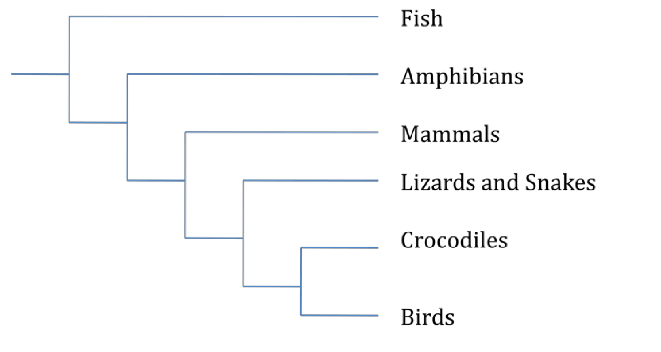
\includegraphics[width=0.9\columnwidth]{figs/imageQ28.png}
    \caption{Phylogenetic tree}
    \label{fig:q28-phylogeny}
\end{figure}

\begin{multicols}{2}
\begin{enumerate}
\item Crocodiles are more closely related to birds than to the other reptiles
\item Fish, lizards and snakes have a common ancestor
\item Mammals and reptiles have evolved from amphibians
\item Mammals are more closely related to crocodiles than to amphibians
\end{enumerate}
\end{multicols}

\item Assume that the abundance of a species in a community is proportional to the size of its niche. As each new species colonises this community, an existing niche is split. The resultant relative abundances of species in this community will be most uneven if:\hfill {(GATE EE 2025)}
\begin{multicols}{2}
\begin{enumerate}
\item The largest niche is always split when a new species colonises
\item The niches are split at random, independent of their size
\item The probability of a niche being split is proportional to its size
\item The smallest niche is always split when a new species colonises
\end{enumerate}
\end{multicols}

\end{enumerate}
\newpage
\fancyhead[C]{Ecology -- EY}

\begin{enumerate}[leftmargin=*,label=\textbf{Q.\arabic*},resume]

\item To study colour preference in bees, a student uses artificial flowers with a sugar reward. She gives bees a choice between blue round flowers and yellow square flowers of the same size. She finds that bees choose the blue flowers significantly more often than the yellow flowers and concludes that bees have a colour preference for blue flowers. However, her friend disagrees and suggests that she should have done the experiment differently. Which of the following would have been more appropriate to test for colour preference in bees?\hfill {(GATE EE 2025)}
\begin{multicols}{2}
\begin{enumerate}
\item choice between blue round and blue square flowers
\item choice between blue round and yellow round flowers
\item choice between yellow round and blue square flowers
\item choice between yellow round and yellow square flowers
\end{enumerate}
\end{multicols}

\item Which of the following does NOT form a component of phytohormone action?\hfill {(GATE EE 2025)}
\begin{multicols}{2}
\begin{enumerate}
\item recognition of specific proteins
\item regulation of gene activity
\item splitting of water molecules
\item signal transduction across the cell
\end{enumerate}
\end{multicols}

\item The following three panels show the change in population size over time for two species when they are found alone and when they are found together. Which kind of interaction best describes the relationship between the two species?\hfill {(GATE EE 2025)}

\begin{figure}[H]
    \centering
    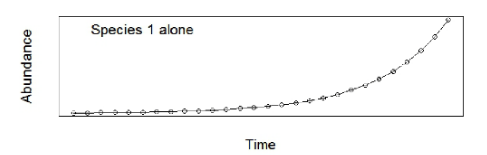
\includegraphics[width=0.9\columnwidth]{figs/ImageQ32a.png}  
    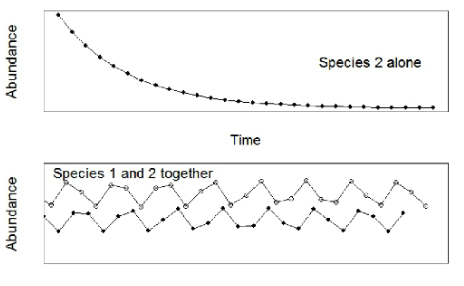
\includegraphics[width=0.9\columnwidth]{figs/ImageQ32b.png}
    \caption{Change in population size over time for Species 1 and 2}
    \label{fig:q32-panel}
\end{figure}


\begin{multicols}{2}
\begin{enumerate}
\item Amensalism
\item Competition
\item Mutualism
\item Predation
\end{enumerate}
\end{multicols}

\item Fresh water fish belonging to the family Galaxoidae are found exclusively in the southern parts of the continents of South America, Africa and Australia. This pattern is explained by the theory proposed by:\hfill {(GATE EE 2025)}
\begin{multicols}{2}
\begin{enumerate}
\item Alfred Russel Wallace
\item Alfred Wegener
\item Charles Darwin
\item Charles Lyell
\end{enumerate}
\end{multicols}

\item Ant species X preys upon ant species Y. A researcher has the following set of observations regarding the behaviour of species X where aggression signifies a predatory response.

\begin{center}
\begin{tabular}{ll}
    \textbf{Group I} & \textbf{Group II} \\
    P. Ferrite & 1. Hexagonal Close Packed (HCP) \\
    Q. Austenite & 2. Body Centered Cubic (BCC) \\
    R. Martensite & 3. Body Centered Tetragonal (BCT) \\
    & 4. Face Centered Cubic (FCC)
\end{tabular}
\end{center}


Which of the following statement(s) are correct regarding the behaviour of Species X?\hfill {(GATE EE 2025)}
\begin{multicols}{2}
\begin{enumerate}
\item i, ii
\item ii, iv
\item i, iii
\item iii, iv
\end{enumerate}
\end{multicols}

\item In the schematic below, the left panel represents climatic zones occupied by two different biomes, X and Y, along gradients of temperature and precipitation. The right panel depicts the expected species-area relationships of these two biomes. From the figures below, which of the following are most likely to be true?\hfill {(GATE EE 2025)}
\begin{figure}[H]
  \centering
  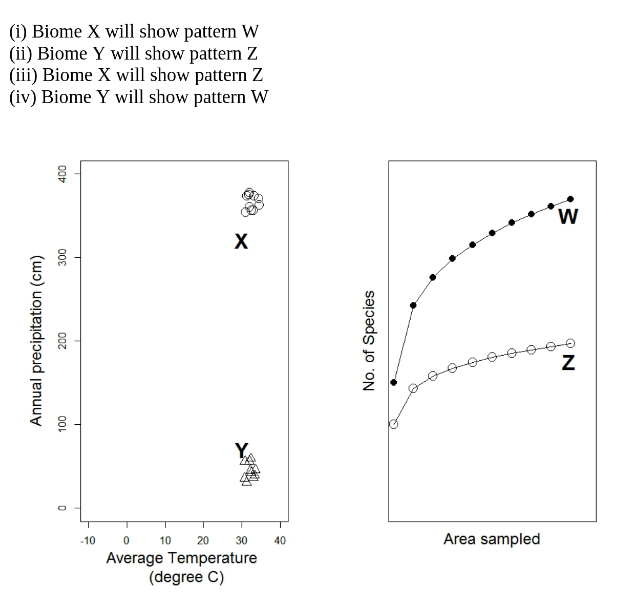
\includegraphics[width=0.9\columnwidth]{figs/imageQ35.png}
  \caption{Schematic Q35.}
  \label{fig:q35-schematic}
\end{figure}


\begin{multicols}{2}
\begin{enumerate}
\item i and ii
\item i and iv
\item ii and iii
\item iii and iv
\end{enumerate}
\end{multicols}

\item In many plant and animal communities found on islands, the number of species ($S$) changes with the area ($A$) of the island as follows: $S = c A^z$, where $0 < z < 1$ and $c>0$. Which graph best represents such species-area relationship?\hfill {(GATE EE 2025)}


\begin{figure}[H]
    \centering
    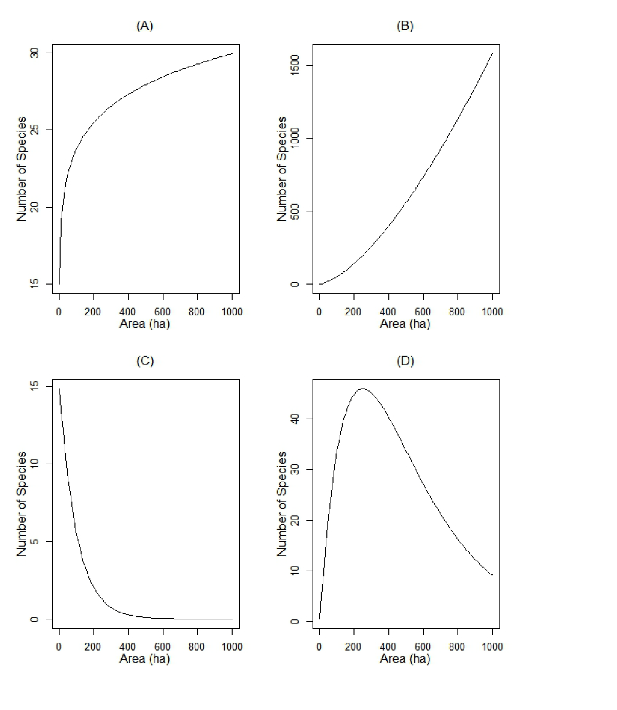
\includegraphics[width=0.9\columnwidth]{figs/imageQ36.png}
    \caption{Graphs}
    \label{fig:q36-graphs}
\end{figure}


\rule{7cm}{0.15mm}

\item Males in a population differ in time spent displaying to females. A researcher hypothesizes predators cause these differences: males display longer in absence of predators and shorter when predators nearby. Which study design is most appropriate?\hfill {(GATE EE 2025)}
\begin{multicols}{2}
\begin{enumerate}
\item Map predator distribution and female abundance; quantify male display variation without predators.
\item Measure display rates, remove predators, measure again, repeat across populations.
\item Measure display rates in areas with/without predators; capture males, switch areas, measure display.
\item Measure display rates in areas with/without predators; manipulate female presence, measure display.
\end{enumerate}
\end{multicols}

\item In Batesian mimicry, a harmless species mimics a harmful or toxic model species. Increasing relative abundance of the mimic will:\hfill {(GATE EE 2025)}
\begin{multicols}{2}
\begin{enumerate}
\item negatively affect both model and mimic populations
\item negatively affect the model but not the mimic population
\item positively affect both model and mimic populations
\item positively affect the mimic but not the model population
\end{enumerate}
\end{multicols}

\item There are two alleles at a locus in a population in Hardy-Weinberg equilibrium. If proportion of dominant phenotype is 0.99, what proportion of the population is heterozygous?
\hfill {(GATE EE 2025)}
\rule{4cm}{0.15mm}

\item Haemophilia is a sex-linked recessive trait causing bleeding disorders. In a family with three children, the two sons have haemophilia, parents normal. Probability daughter inherited gene? And probability afflicted?\hfill {(GATE EE 2025)}
\begin{multicols}{2}
\begin{enumerate}
\item $\frac{1}{2}$, 0
\item $\frac{1}{2}$, 1
\item $\frac{1}{2}$, $\frac{1}{4}$
\item $\frac{1}{4}$, 0
\end{enumerate}
\end{multicols}

\end{enumerate}

\begin{enumerate}[leftmargin=*,label=\textbf{Q.\arabic*},resume]

\item Which of the graphs below represents the relationship between population size ($N$) and population growth rate ($dN/dt$) for a population showing exponential growth?\hfill {(GATE EE 2025)}

\rule{8cm}{0.15mm}

\begin{figure}[H]
    \centering
    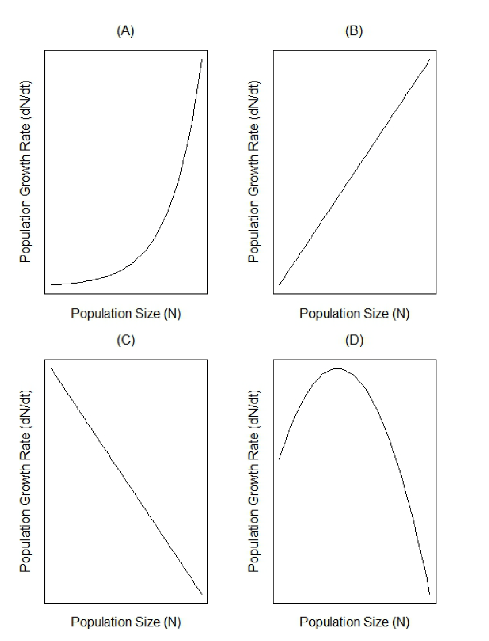
\includegraphics[width=0.9\columnwidth]{figs/imageQ41.png}
    \caption{Population Growth Rate vs Population Size}
    \label{fig:q41-graph}
\end{figure}

\item Two islands, P and Q, are similar in habitat and other features. They are 100 and 200 km$^2$ in size respectively, but have the same number of species. Which of the following statements can independently explain this observation? \hfill {(GATE EE 2025)}
\begin{multicols}{2}
\begin{enumerate}
\item P is closer to the mainland than Q and P has lower speciation rates
\item P is closer to the mainland than Q and P has higher speciation rates
\item P is further away from the mainland than Q and P has higher speciation rates
\item P is further away from the mainland than Q and P has lower speciation rates
\end{enumerate}
\end{multicols}

\item In reverse sexual selection, variance in mating success is higher in females than in males. In such species, which of the following is most expected?\hfill {(GATE EE 2025)}
\begin{multicols}{2}
\begin{enumerate}
\item Females are the competing sex and males are the choosy sex
\item Males are the competing sex and females are the choosy sex
\item Mating is random and both sexes are not choosy
\item Mating is non-random and both sexes are equally choosy
\end{enumerate}
\end{multicols}

\item According to the Hamilton-Zuk hypothesis, females prefer males with the most elaborate ornaments because those ornaments signal parasite resistance. Which of the following is NOT an assumption of this hypothesis?\hfill {(GATE EE 2025)}
\begin{multicols}{2}
\begin{enumerate}
\item Parasites reduce male fitness
\item Parasite resistance is indicated by male ornamentation
\item Parasite resistance is genetic
\item Parasite load is positively correlated with male ornamentation
\end{enumerate}
\end{multicols}

\item A plant produces flowers that are open through the day and the night. An experimenter places pollen on the stigmas of freshly opened flowers and covers them after pollination to prevent natural pollinators from having access to the flowers. When experimental pollination was carried out during the day, 40\% of the flowers yielded fruit. When experimental pollination was carried out during the night, 80\% of the flowers yielded fruit. However, when flowers were kept open to natural pollination during the day (covered at night), 35\% of flowers produced fruit. 20\% of flowers exposed to natural pollination during the night (covered during the day) produced fruit. Which of the following statements is NOT a plausible explanation of these results?\hfill {(GATE EE 2025)}
\begin{multicols}{2}
\begin{enumerate}
\item night pollinators are low in abundance
\item night pollinators are abundant
\item night pollinators are low in pollination efficiency
\item pollinators are active during the day
\end{enumerate}
\end{multicols}

\item Sex is determined by temperature in many reptiles, including crocodiles and turtles. While lower temperatures produce males in turtles, the pattern is the opposite in crocodiles. Due to climate change, there is an increase in temperatures which results in a change in sex ratios. In small populations, this change in demography is likely to negatively impact the population growth of:\hfill {(GATE EE 2025)}
\begin{multicols}{2}
\begin{enumerate}
\item crocodiles more than turtles
\item neither of the two species
\item both species equally
\item turtles more than crocodiles
\end{enumerate}
\end{multicols}

\item An unbiased coin is tossed four times. What is the probability of getting at least three "heads" in a row? \hfill {(GATE EE 2025)}

\rule{4cm}{0.15mm}

\item In a study of interactions between plants, ants and caterpillars, the following experimental treatments were imposed: i) Control (both ants and caterpillars are present); ii) Ant removal; iii) Caterpillar removal; iv) Ant and caterpillar removal. Plus (+) indicates presence and minus (-) indicates absence on plants. The results for plant performance (growth) from this experiment are shown in the figure below. Plant performance in all treatments were significantly different from each other. Based on these results, which of the following inferences is correct?\hfill {(GATE EE 2025)}

\begin{figure}[H]
    \centering
    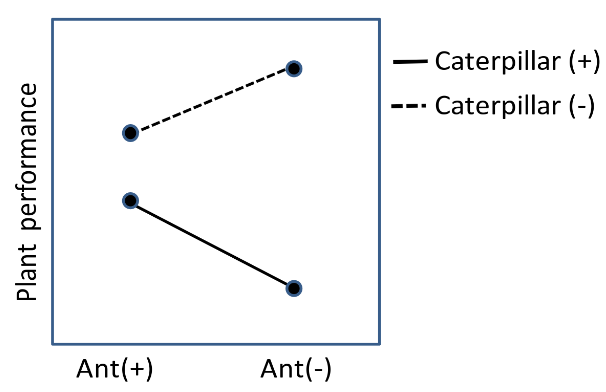
\includegraphics[width=0.9\columnwidth]{figs/imageQ48.png}
    \caption{Plant performance under different ant and caterpillar treatments}
    \label{fig:q48-performance}
\end{figure}

\begin{multicols}{2}
\begin{enumerate}
\item In the absence of caterpillars, ants negatively affected plant performance
\item In the absence of ants, caterpillars positively affected plant performance
\item In the presence of caterpillars, ants negatively affected plant performance
\item In the presence of ants, caterpillars positively affected plant performance
\end{enumerate}
\end{multicols}

\item Both males and females of a fish species show variation in colour. A population of this species consists of 40\% blue females, 20\% red females, 20\% blue males and 20\% red males. A researcher catches one fish at random from this population. Given that a male fish is caught, the probability that it is blue is\hfill {(GATE EE 2025)} \rule{4cm}{0.15mm}.

\rule{4cm}{0.15mm}

\item Assume that an asexually propagating fungus has three colors of colonies, white, black and red. Such variability in color may have originated due to:\hfill {(GATE EE 2025)}
\begin{multicols}{2}
\begin{enumerate}
\item germline mutation
\item heterokaryosis
\item genetic linkage
\item sexual cross-over
\end{enumerate}
\end{multicols}

\item Shannon's index of diversity is calculated using the equation below, where $p_i$ is the proportion of the $i^{th}$ species and $\ln$ is natural logarithm. For a community with a given number of species, which of the following statements is true?\hfill {(GATE EE 2025)}
\begin{multicols}{2}
\begin{enumerate}
\item Shannon's index will be highest if all species have equal abundance
\item Shannon's index will be highest if one species is highly dominant
\item Shannon's index will be highest if there are many rare species
\item The relative abundance is irrelevant to Shannon's index
\end{enumerate}
\end{multicols}

\item The schematic below shows the relationship between survivorship with age (relative to maximum lifespan) in Species 1 (dashed line) and Species 2 (solid line). Which of the following inferences is compatible with this figure?\hfill {(GATE EE 2025)}

\begin{figure}[H]
    \centering
    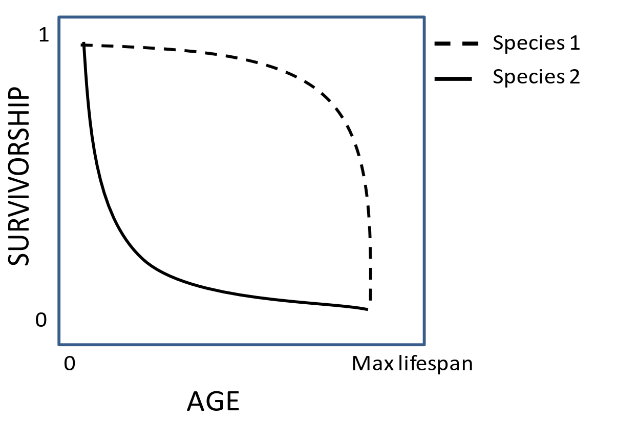
\includegraphics[width=0.9\columnwidth]{figs/imageQ52.png}
    \caption{Survivorship vs Age}
    \label{fig:q52-scbematic}
\end{figure}



\item A team of conservation biologists, surveying a population of frogs on an island, captured and marked 312 individuals in the first sample. In a second sampling, 3 days later, the team caught 140 individuals of which 26 were previously marked. The total number of frogs on the island is estimated to be \rule{4cm}{0.15mm}.\hfill {(GATE EE 2025)}

\rule{4cm}{0.15mm}

\item The following equation represents a hypothetical relationship between fitness ($w$) and shoot:root ratio ($r$) in individuals of a plant species: $w = 10r-10r^2$. At what value of shoot:root ratio ($r$), do these plants achieve maximum fitness?
\hfill {(GATE EE 2025)}
\rule{4cm}{0.15mm}

\item The relative abundance of C3 relative to C4 plant species increases with latitude because of the associated temperature gradient. A study in North America found that at 42\degree North, C3 plants become more abundant than C4 plants. Given an increase in mean global temperatures by 10\degree and no other changes in environmental conditions, the latitude at which C3 plants become more abundant:\hfill {(GATE EE 2025)}
\begin{enumerate}
\item will move Northwards towards the polar region
\item will move Southwards towards the equator
\item will move South of the equator
\item will not change in response to temperature
\end{enumerate}
\begin{center}
  \textbf{END OF QUESTION PAPER}  
\end{center}
\end{enumerate}
\begin{tabular}{|c|c|c|}
     \hline
     \textbf{Mineral} & \textbf{Modal abundance \brak{\%}} & \textbf{Partition coefficient}\\
     \hline
     Clinopyroxene & $45$ & $0.506$ \\
      \hline
      Orthopyroxene & $40$ & $0.42$ \\
      \hline
      Olivine & $10$ & $0.045$ \\
      \hline
      Plagioclase & $05$ & $0.019$ \\
      \hline
\end{tabular}

\end{document}
